\documentclass[12pt]{article}

%\usepackage{fullpage}
%\usepackage[top=1in, bottom=1in, left=1in, left=1in, right=1in]{geometry}
\usepackage[margin=1in, paperwidth=8.5in, paperheight=11in]{geometry}
\usepackage{graphicx}
\usepackage{subcaption}
\usepackage{listings}
\usepackage{color}

\definecolor{dkgreen}{rgb}{0,0.6,0}
\definecolor{gray}{rgb}{0.5,0.5,0.5}
\definecolor{mauve}{rgb}{0.58,0,0.82}

\lstset{frame=tb,
  language=Java,
  aboveskip=3mm,
  belowskip=3mm,
  showstringspaces=false,
  columns=flexible,
  basicstyle={\small\ttfamily},
  numbers=none,
  numberstyle=\tiny\color{gray},
  keywordstyle=\color{blue},
  commentstyle=\color{dkgreen},
  stringstyle=\color{mauve},
  breaklines=true,
  breakatwhitespace=true,
  tabsize=3
}

\begin{document}

\title{UT Machine Learning: HomeWork 2}
\author{Mohamad amin Katebsaber}
\date{\today}
\maketitle

\section{Problem 5 summary}
Figure \ref{fig:mean_nvp} illustrates the distribution of NVP feature which is considered as regression target in our problem set. According to this plot one can deduct that most of our data can almost be clustered in two categories. This deduction proves that we can plot the whole data using PCA technique.


\begin{figure}[h!]
  \centering
  \begin{subfigure}[b]{0.7\linewidth}
    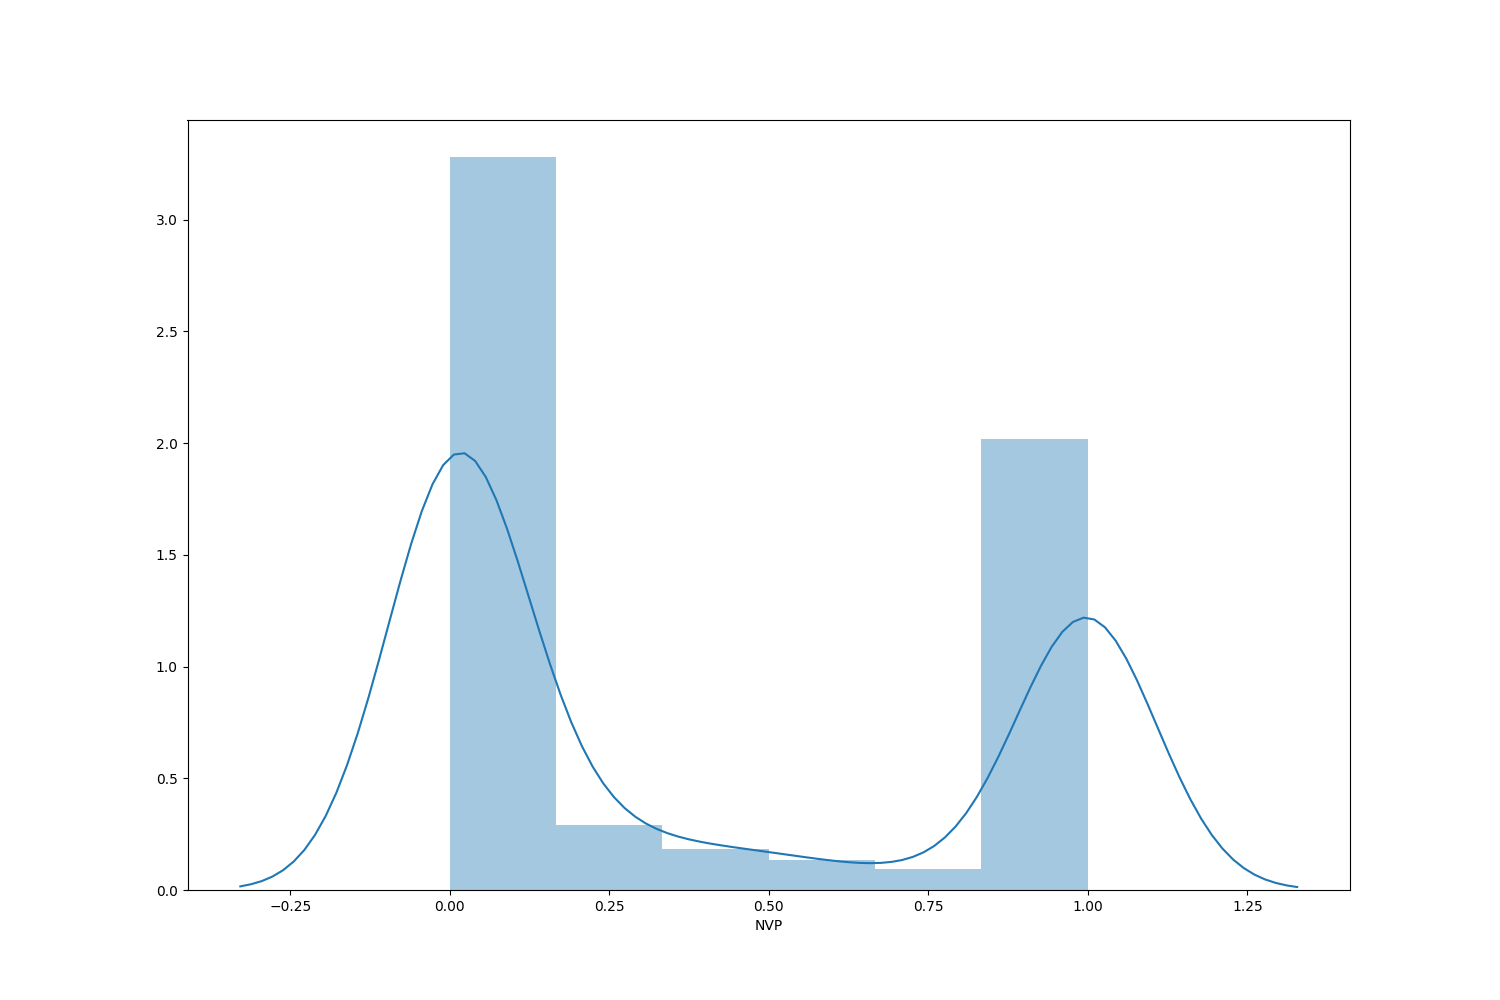
\includegraphics[width=\linewidth]{./plots/mean_NVP.png}    
  \end{subfigure} 
  \caption{Distribution of NVP field}
  \label{fig:mean_nvp}
\end{figure}


Figure \ref{fig:pca} shows the data plotted using two calculated components of PCA. Observations prove our initial hypothesis that the data is clustered in two groups; Subsequently there is a possibility to address this problem in a classification framework but as the question demands, we continue in a regression framework.

As the question states, we have to use Multivariate linear regression, Ridge and LASSO. Results from applying aforementioned algorithms (with $\alpha$ parameters: $100 for Ridge and 0.001 for LASSO$) on the whole dataset is shown in following block:


\begin{lstlisting}

 Multivariate linear regression model

Number of used coefficients: 219
R squared Score: -2.858706063278099e+21
Mean Absolute Error: 1055112737.1771085
Mean Squared Error: 5.7555691297568686e+20
Root Mean Squared Error: 23990767244.414818

 Ridge regression model

Number of used coefficients: 219
R squared test Score: 0.5793774720087499
Mean Absolute Error: 0.24082586437752515
Mean Squared Error: 0.08468593775642133
Root Mean Squared Error: 0.2910084839938886

 Lasso regression model

Number of used coefficients: 63
R squared test Score: 0.6744580726645737
Mean Absolute Error: 0.18791821976331105
Mean Squared Error: 0.0655429073832366
Root Mean Squared Error: 0.25601349062742107
\end{lstlisting}


\begin{figure}[h!]
  \centering
  \begin{subfigure}[b]{0.7\linewidth}
    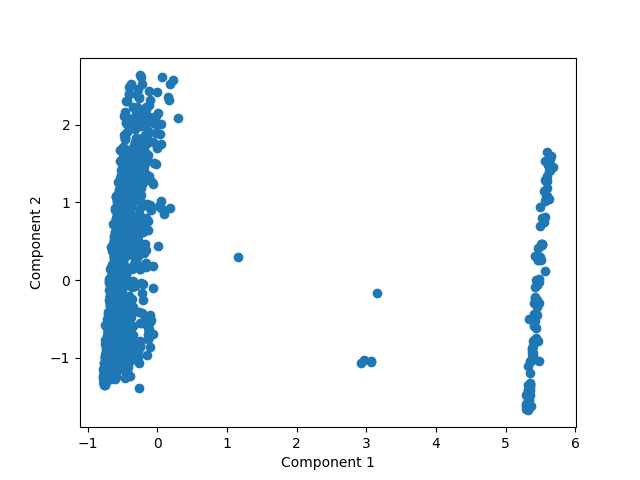
\includegraphics[width=\linewidth]{./plots/c1-c2.png}    
  \end{subfigure} 
  \caption{PCA with two components over data}
  \label{fig:pca}
\end{figure}


Next block of results, shows the outputs of applying algorithms on initial 50 samples of dataset.


\begin{lstlisting}
 Multivariate linear regression model

Number of used coefficients: 125
R squared Score: -0.0865482085770819
Mean Absolute Error: 0.3661537717841558
Mean Squared Error: 0.2187599280531736
Root Mean Squared Error: 0.46771778676160436

 Ridge regression model

Number of used coefficients: 120
R squared test Score: 0.09748593118386495
Mean Absolute Error: 0.39903892985285944
Mean Squared Error: 0.18170745780322944
Root Mean Squared Error: 0.42627157752215833

 Lasso regression model

Number of used coefficients: 51
R squared test Score: 0.1530951544250253
Mean Absolute Error: 0.3099673082411051
Mean Squared Error: 0.17051138791944567
Root Mean Squared Error: 0.41293024582784643
\end{lstlisting}

A glimpse to the results (Total samples and 50 initial samples), demonstrate the superiority of Lasso over Ridge and Multivariate regression since the R squared score is higher in this model. However a closer look, shows that the Lasso model was able to achieve this comparable result by only utilizing approximately $40\%$ of coefficients used by other models (Compare number of used coefficients in the result boxes).

Addition of feature products (P1*P2, P1*P3, P1*P4 and etc) as new features, increased R squared score about $14\%$ -training on the whole dataset- as shown in following box.
\begin{lstlisting}
 Multivariate linear regression model

Number of used coefficients: 12347
R squared Score: -8.213881354439473e+18
Mean Absolute Error: 435603297.01152885
Mean Squared Error: 1.6537398708591306e+18
Root Mean Squared Error: 1285978176.6651917

 Ridge regression model

Number of used coefficients: 12109
R squared test Score: 0.7152238542745143
Mean Absolute Error: 0.18155617142118535
Mean Squared Error: 0.05733533832958122
Root Mean Squared Error: 0.239447986689346

 Lasso regression model

Number of used coefficients: 282
R squared test Score: 0.7982564852964698
Mean Absolute Error: 0.1384875055133704
Mean Squared Error: 0.040617983089341905
Root Mean Squared Error: 0.20153903614273316
\end{lstlisting}

Figure \ref{fig:benchmark} demonstrates the overall performance of models.
\begin{figure}[h!]
  \centering
  \begin{subfigure}[b]{0.4\linewidth}
    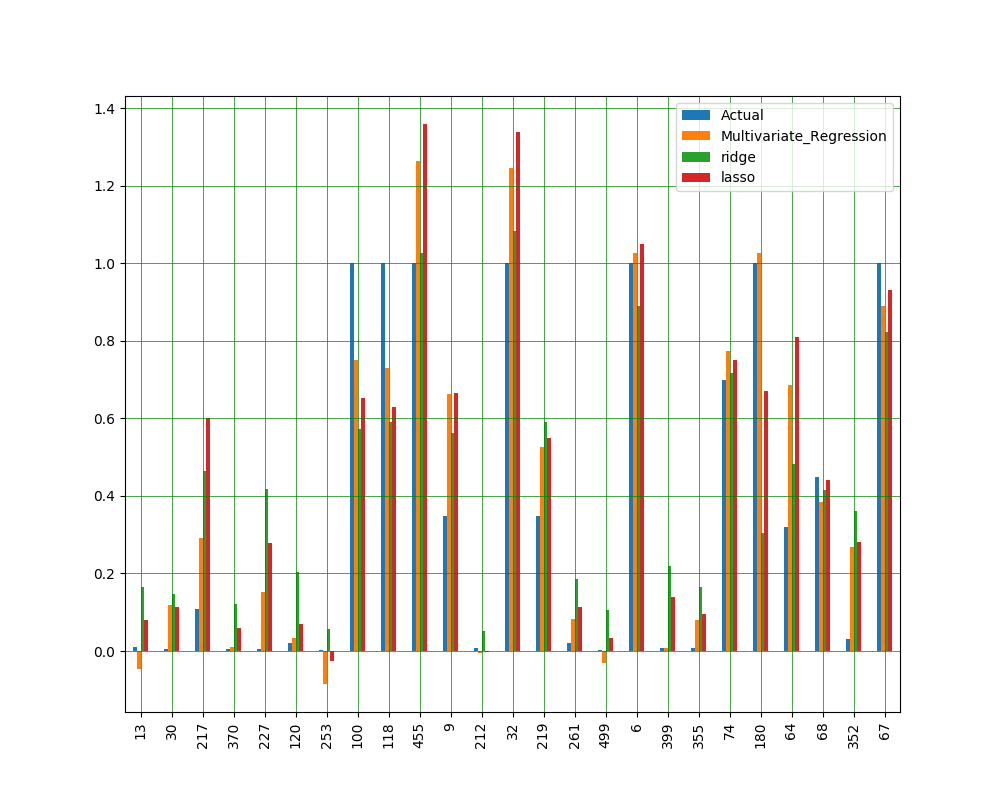
\includegraphics[width=\linewidth]{./plots/actual_predicted_difference.png}
    \caption{Prediction using models trained on the whole dataset}
  \end{subfigure} 
  \begin{subfigure}[b]{0.4\linewidth}
    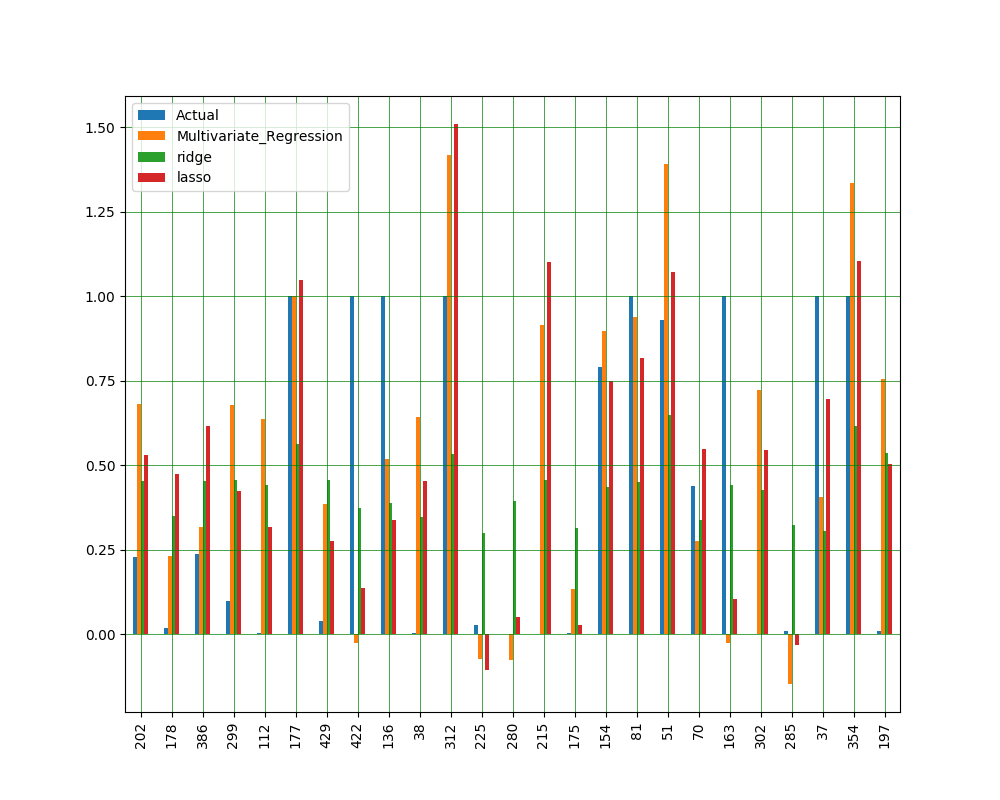
\includegraphics[width=\linewidth]{./plots/actual_predicted_difference_50.png}
    \caption{Prediction using models trained on 50 initial records}
  \end{subfigure}
  \caption{Model benchmarks: X axis is the sample identifier of the record in dataset and Y axis illustrates the real and predicted value for the record. Note that NVP values are normalized between 0 and 1.}
  \label{fig:benchmark}
\end{figure}
\end{document}